% Created 2018-11-02 Fri 15:56
% Intended LaTeX compiler: pdflatex
\documentclass[11pt]{article}
\usepackage[utf8]{inputenc}
\usepackage[T1]{fontenc}
\usepackage{graphicx}
\usepackage{grffile}
\usepackage{longtable}
\usepackage{wrapfig}
\usepackage{rotating}
\usepackage[normalem]{ulem}
\usepackage{amsmath}
\usepackage{textcomp}
\usepackage{amssymb}
\usepackage{capt-of}
\usepackage{hyperref}
\usepackage{color}
\usepackage{minted}
\usepackage[margin=2cm]{geometry}
\author{John Harwell}
\date{\today}
\title{}
\begin{document}

\begin{center}
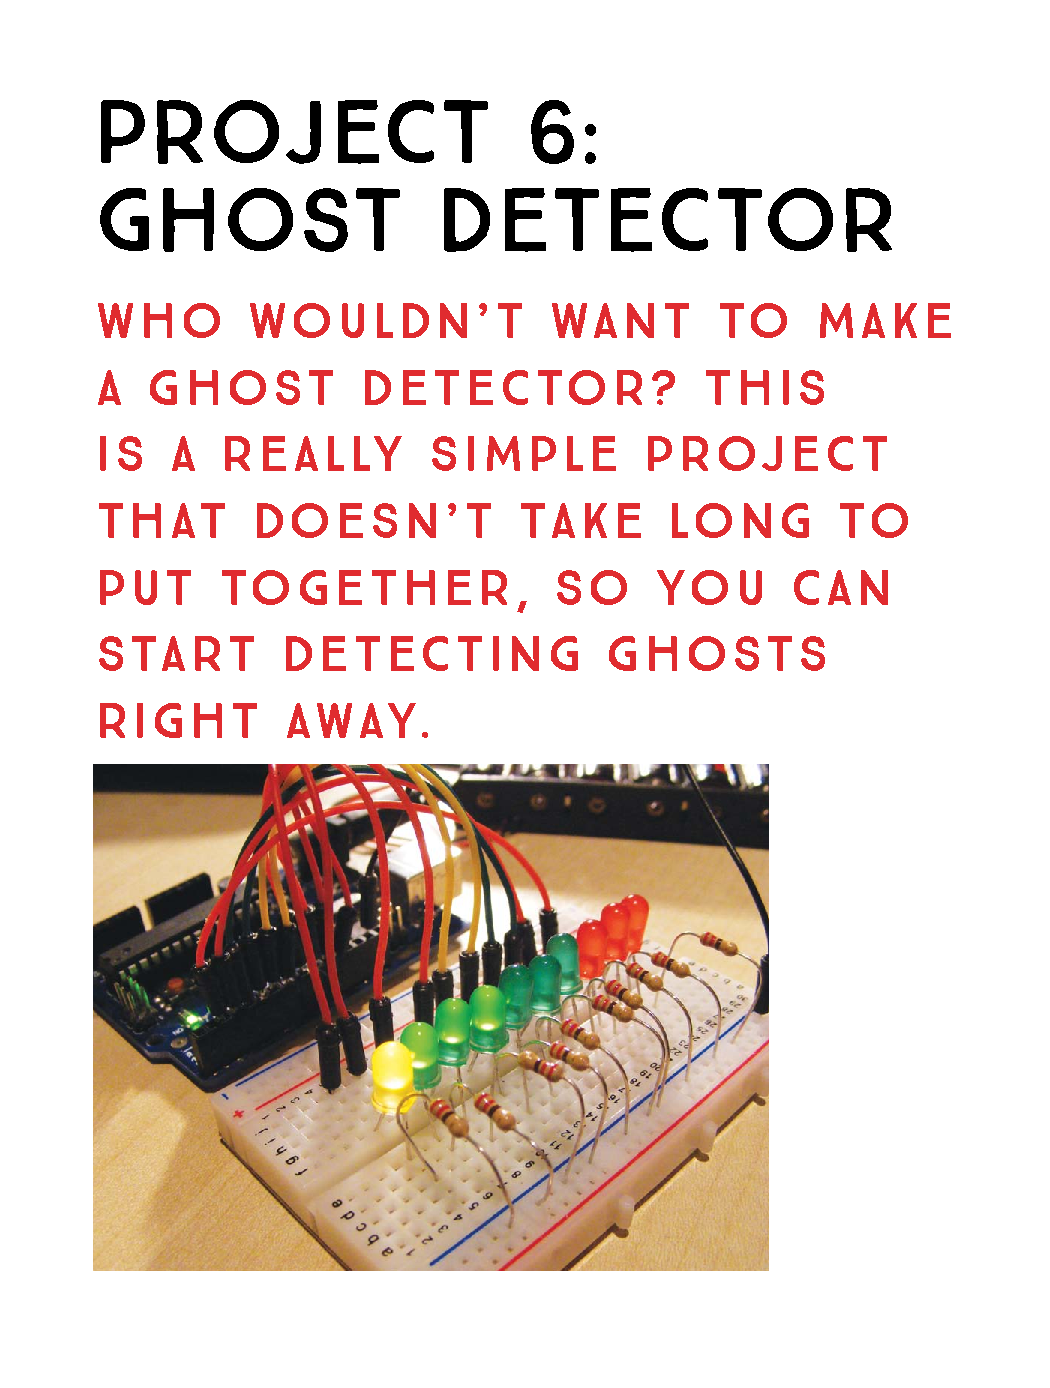
\includegraphics[width=.9\linewidth]{./exp3-ghost-detector1.pdf}
\end{center}

\begin{center}
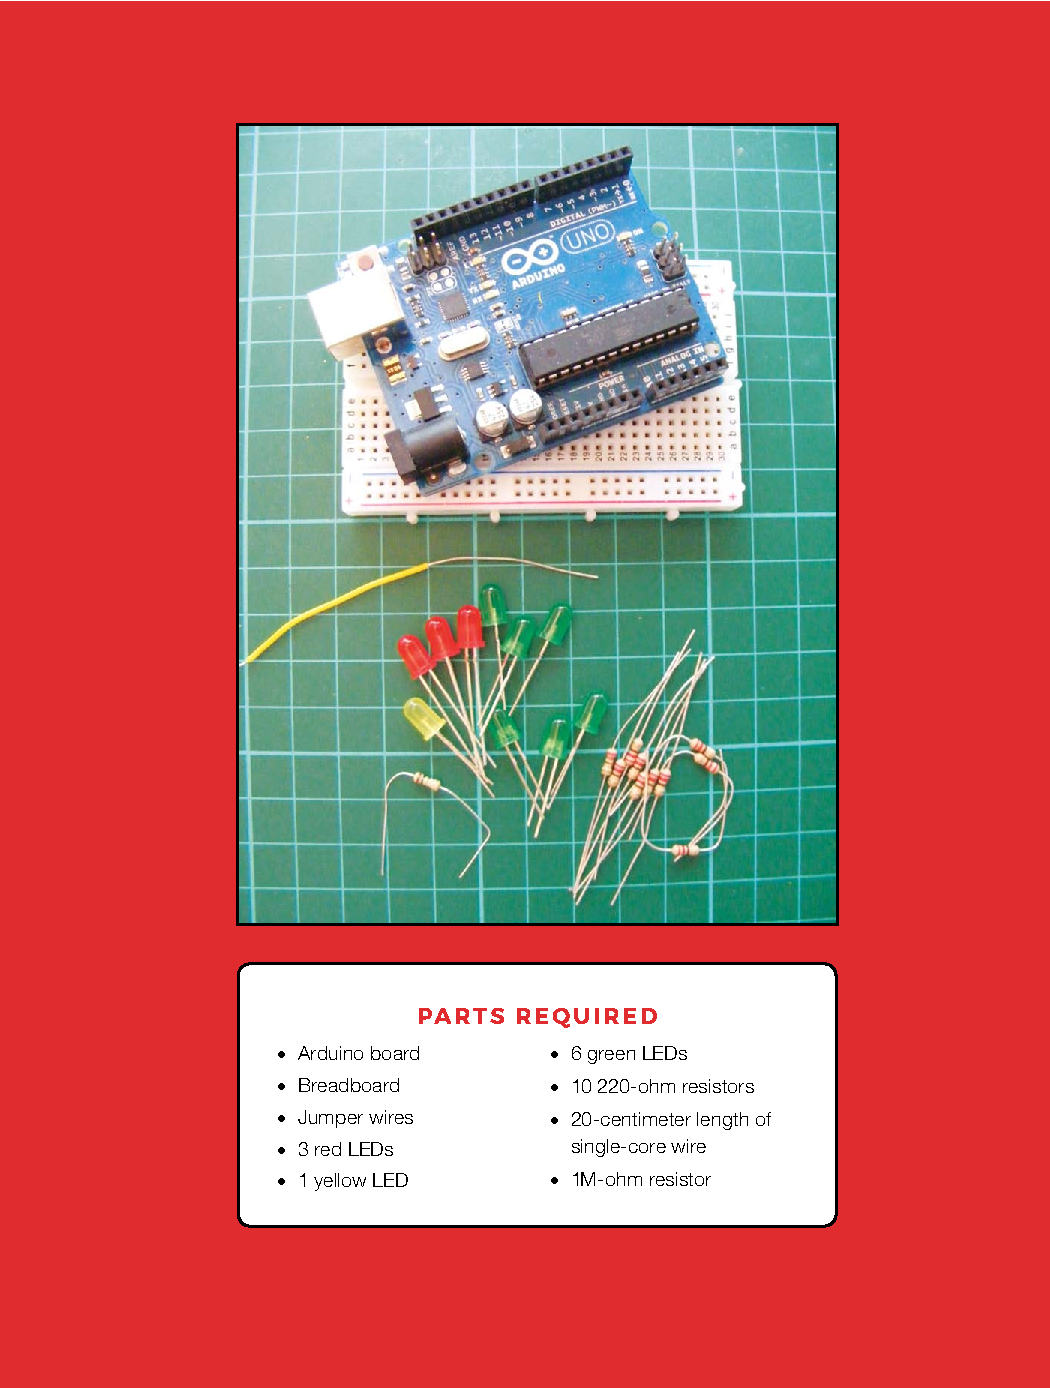
\includegraphics[width=.9\linewidth]{./exp3-ghost-detector2.pdf}
\end{center}

\section{Setup}
\label{sec:org3b90a27}

First you will need to download, unzip, and install the Arduino Integrated Development Environment (IDE) from
\url{https://www.arduino.cc/en/Main/Donate} (does not need admin privileges).

\section{Building The Circuit}
\label{sec:org7659439}

The schematic for the circuit you will be building is below.

\begin{center}
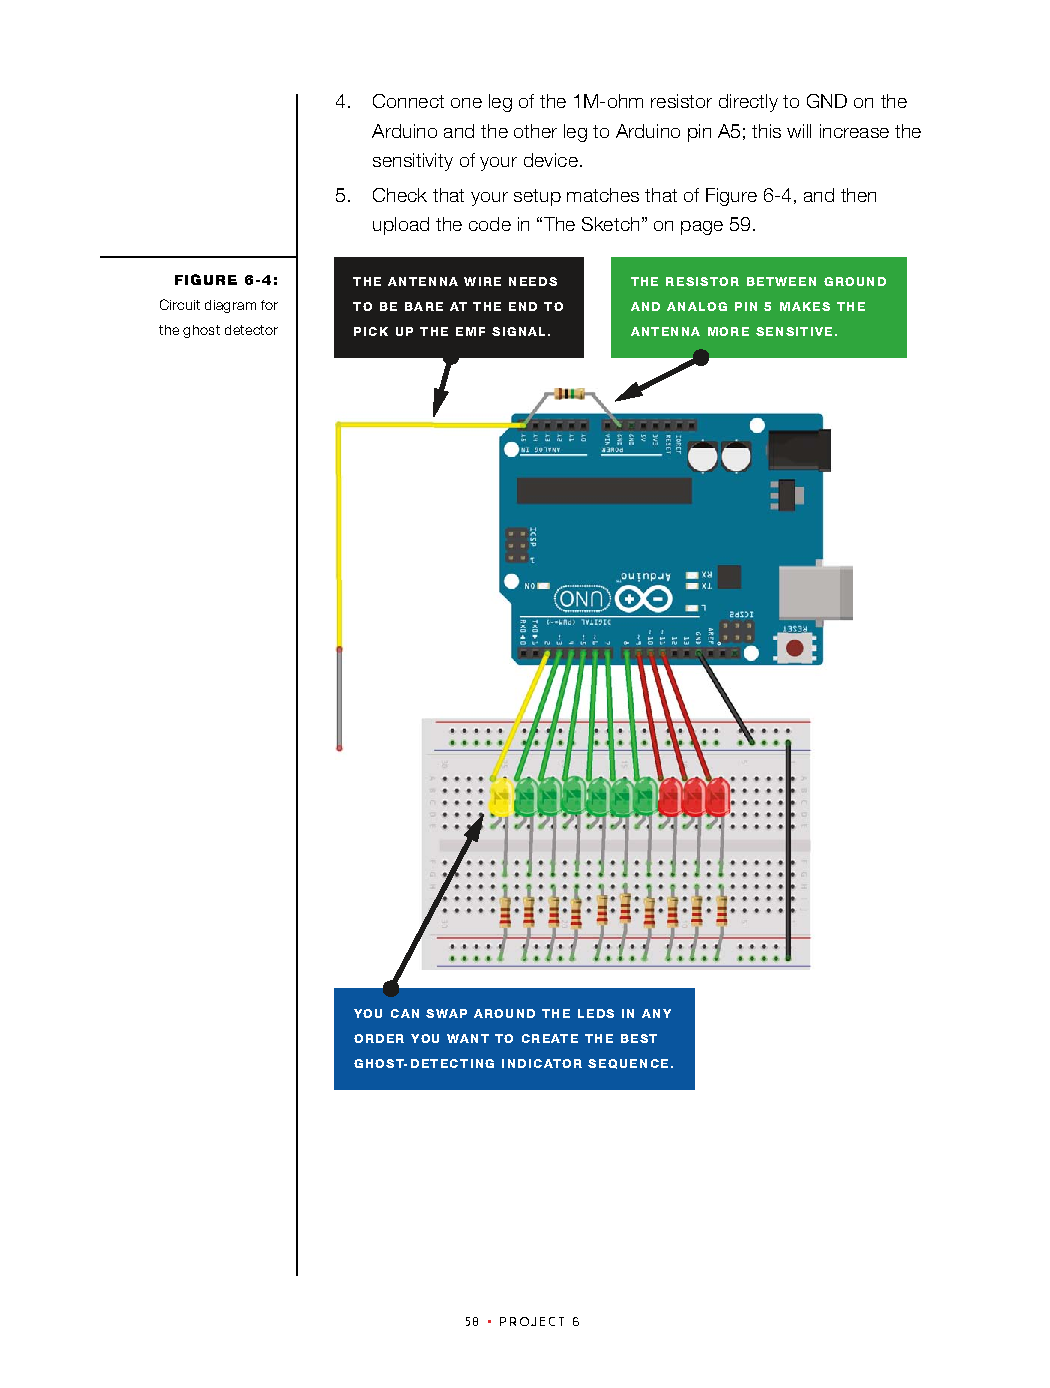
\includegraphics[width=.9\linewidth]{./exp3-ghost-detector6.pdf}
\end{center}

\begin{center}
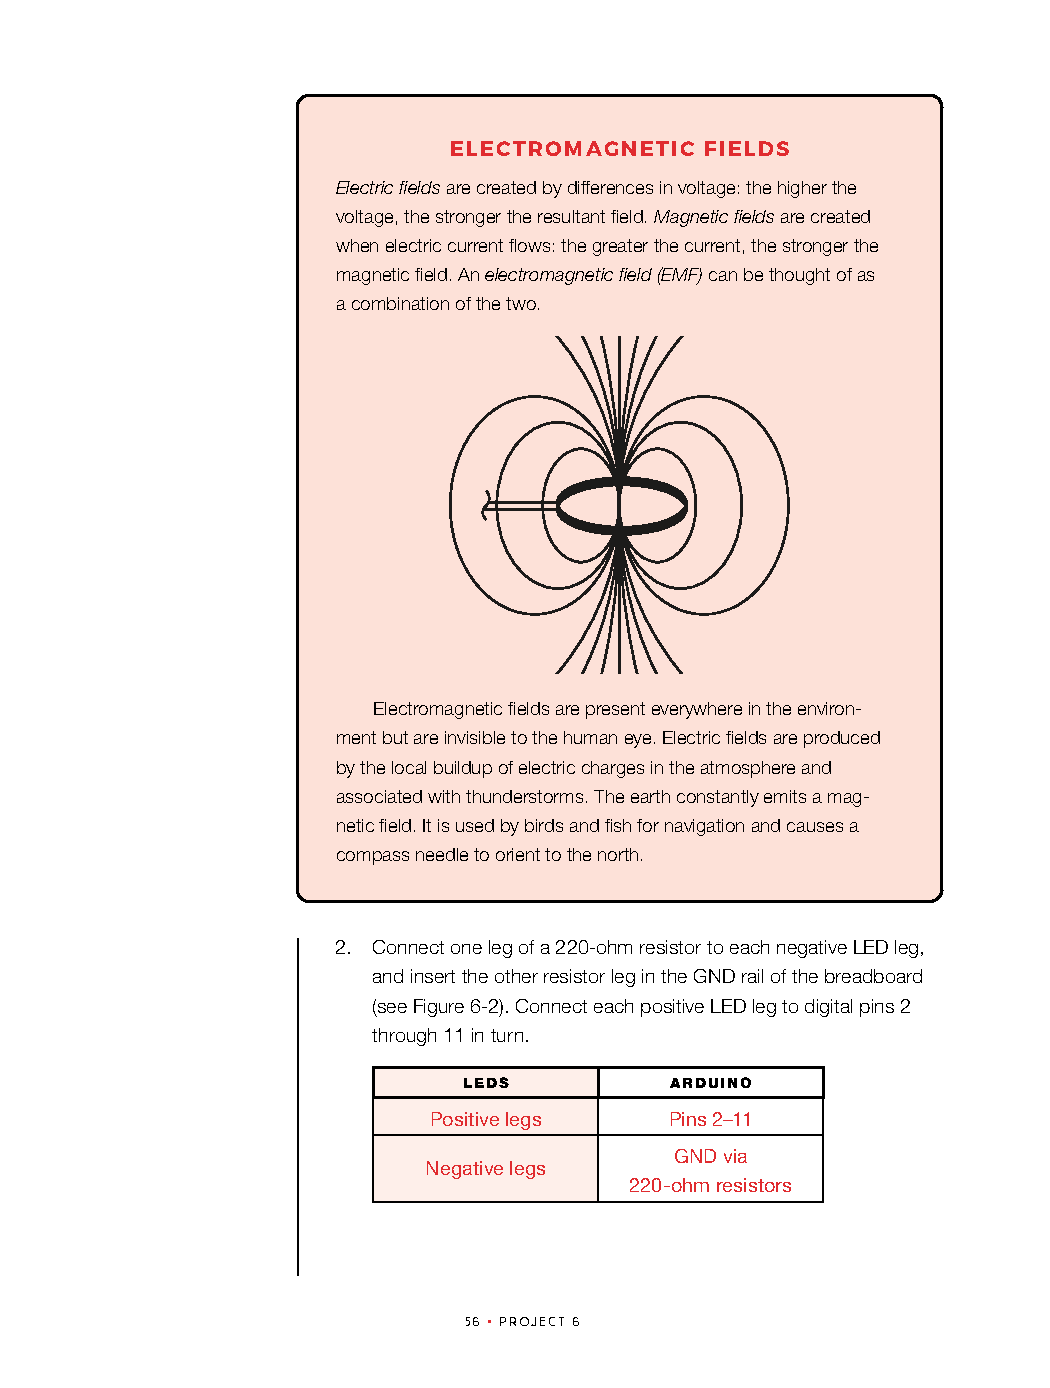
\includegraphics[width=.9\linewidth]{./exp3-ghost-detector4.pdf}
\end{center}

\texttt{PAUSE}

What is a circuit? Why are resistors needed? Why can resistors be placed in any direction in a circuit, but LEDs
only work if they are placed in a certain direction.

\section{Programming the Arduino}
\label{sec:org0f13fc0}

The base code for programming the Arduino is provided. Using the Arduino IDE, open the \texttt{.ino} file.

\texttt{PAUSE}

The IDE allows you to do 4 things: edit the code, verify the code is correct (i.e. does not contain syntax
errors), upload the code to the Arduino, and view the diagnostic output of things as they run on the Arduino.

The bare wire picks up the signal from the electromagnetic fields in the atmosphere and sends a value between 0 and 1023
to the Arduino (this is done by a special kind of circuit, an Analog-to-Digital Converter, or ADC for short ). The base
code evaluates the reading from the analog pin to determine how many LEDs should be on or off in sequence to indicate
the strength of the electromagnetic signal. For example, 1023 would be the highest value, so all LEDs would be lit; a
reading of 550 would light five LEDs. The sketch loops to continuously read the analog input, and the LED lights
constantly move to show the reading. If you find that the EMF readings set off your LED sequence to the maxi- mum level
every time, reduce the senseLimit value to compensate.  The sketch takes an average of 25 number readings each time it
loops through, and uses the average from those readings to mitigate big fluctuations that may cause the LEDs to light up
too quickly.

\texttt{PAUSE}

Can you map each part of the description above to lines in the code?

\section{Tuning The Code}
\label{sec:org9593334}

You may notice that your detector is not that sensitive, or that it is TOO sensitive (i.e. all LEDs are always on). This
can be fixed in the code by changing the thresholds that each LED turns on at. For example, if one additional LED turns
on every time the reading goes up by 100, and that is not sensitive enough, you could make one additional LED turn on
every time the reading goes up by 50 to make it more sensitive.


\section{Extending The Code}
\label{sec:org97f2b16}

Once you have the ghost detector working try adding some sounds via one or more buzzers that beep at increasing speeds
or different patterns depending on the reading. The buzzers we have are called \emph{piezo} buzzers. They are not like a
regular speaker that you might think of. It uses a material that’s piezoelectric, which means it changes shape when you
apply electricity to it. By adhering a piezo-electric disc to a thin metal plate, and then applying electricity, we can
bend the metal back and forth, which in turn creates noise. The faster you bend the material, the higher the pitch of
the noise that’s produced. This rate is called frequency. Again, the higher the frequency, the higher the pitch of the
noise we hear. So basically, by shocking the plate over and over really fast, we can make noise.


You should following the same idea as the LED circuits you built:

\begin{enumerate}
\item Assign a new pin on the Arduino to your new buzzer (such as 12 or 13), and add this definition to the code.
\item The buzzers are similar to LEDs, in that they only work when plugged in a certain way, and they need a resistor
between their negative end and ground.
\item Once you have the circuit built, you are ready to add the buzzer trigger into the code! The functions you will need
are:

\texttt{Tone(int pin, int frequency)}, which controls which pin gets the buzzer signal and what the frequency of the sound
will be.

\texttt{noTone(int pin)}, which turns off the buzzing signal on the specified pin.

Can you figure out how to play a tone when the maximum sensor reading is observed (and all the LEDs are on) ? What
about playing a different tone or pattern depending on what the sensor reading is (i.e. going up in pitch the more
LEDs are on) ?
\end{enumerate}
\end{document}
